\documentclass{beamer}
%Information to be included in the title page:
% \title{Sample title}
% \author{Anonymous}
% \institute{Overleaf}
\usepackage{xcolor}
\usepackage{booktabs}
\usepackage{graphicx}
\usepackage{subcaption}
\usepackage[]{hyperref}
\usepackage{tikz}
\usepackage{ulem}

\usetheme[]{default}
\begin{document}
\renewcommand{\d}{\: \mathrm{d} }
\newcommand{\e}{\mathrm{e}}


\title[] {Recitation Class 8}

\author[lzx]{Zexi Li}

\institute[email]{lzx12138@sjtu.edu.cn}

\date{2021.07.27}

\frame{\titlepage}

\AtBeginSection[]
{
    \begin{frame}
        \frametitle{Table of Contents}
        \tableofcontents[currentsection]
    \end{frame}
}

\begin{frame}
    \frametitle{Outline}
    \tableofcontents
\end{frame}

\section{Chapter 10 - Fundamentals of the Metal–Oxide–Semiconductor Field-Effect Transistor}
    \begin{frame} \frametitle{MOSFET}
        \begin{figure}[H]
            \centering
            \begin{subfigure}[t]{0.45\linewidth}
                \centering
                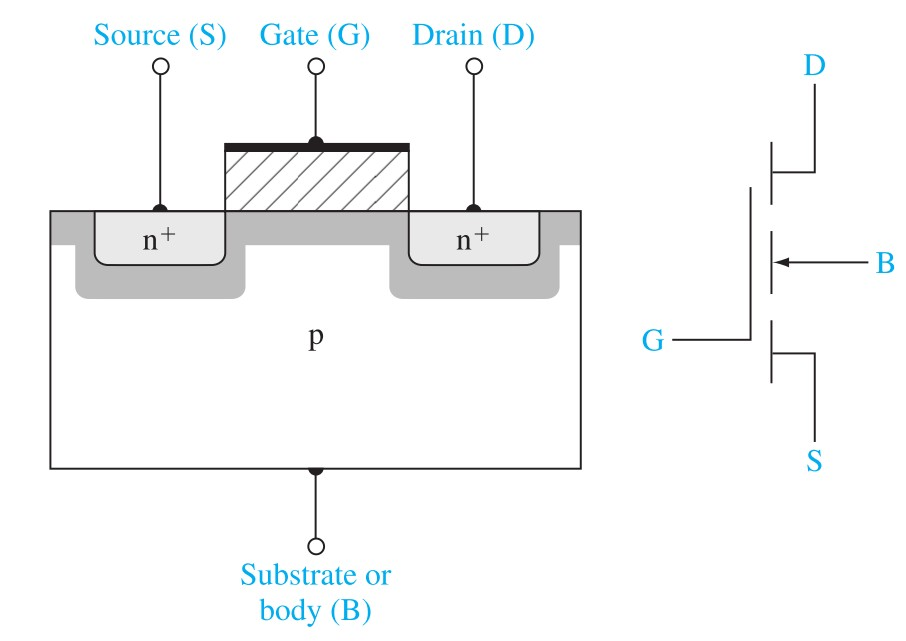
\includegraphics[width=0.9\linewidth]{NMOS-enhancement.jpg}
                \caption{n-channel enhancement MOSFET}
                \label{subfig:NMOS-enhancement.jpg}
            \end{subfigure}
            \begin{subfigure}[t]{0.45\linewidth}
                \centering
                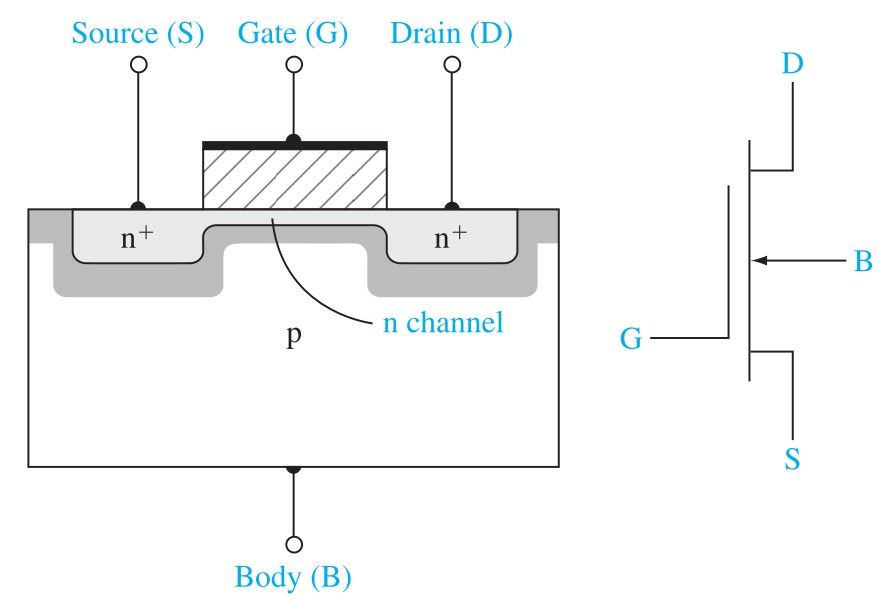
\includegraphics[width=0.9\linewidth]{NMOS-depletion.jpg}
                \caption{n-channel depletion MOSFET}
                \label{subfig:NMOS-depletion.jpg}
            \end{subfigure}
        \end{figure}
        
        \par \textcolor{blue}{Enhancement mode}: the semiconductor substrate is not inverted directly under the oxide with zero gate voltage.
        \par \textcolor{blue}{Depletion mode}: a p-channel region exists under the oxide with $0V$ applied to the gate.
    \end{frame}
    \begin{frame} \frametitle{MOSFET}
        \begin{figure}[H]
            \centering
            \begin{subfigure}[t]{0.45\linewidth}
                \centering
                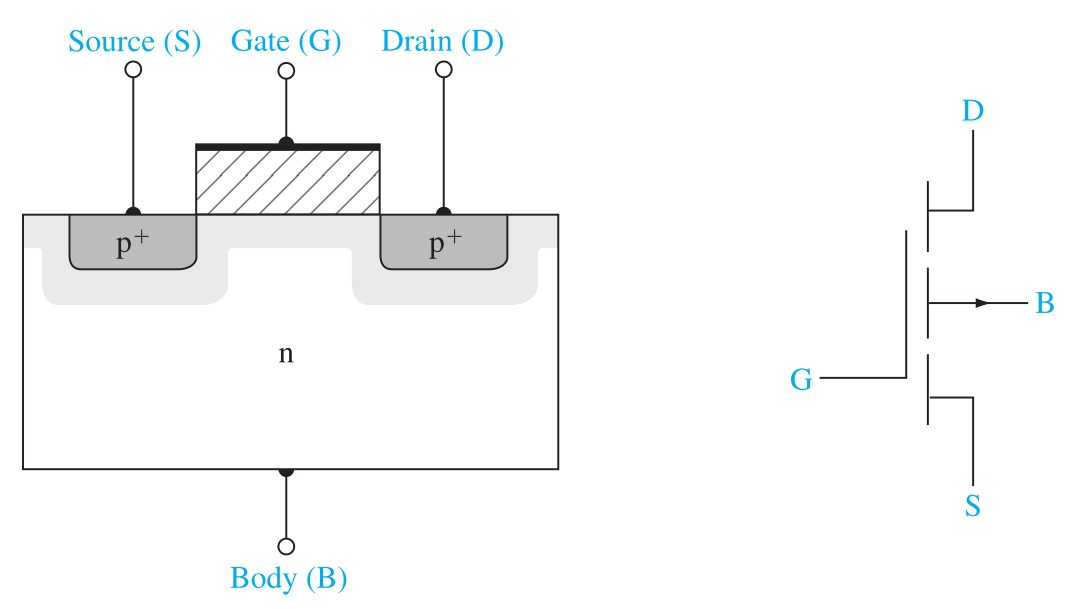
\includegraphics[width=0.9\linewidth]{PMOS-enhancement.jpg}
                \caption{p-channel enhancement MOSFET}
                \label{subfig:PMOS-enhancement.jpg}
            \end{subfigure}
            \begin{subfigure}[t]{0.45\linewidth}
                \centering
                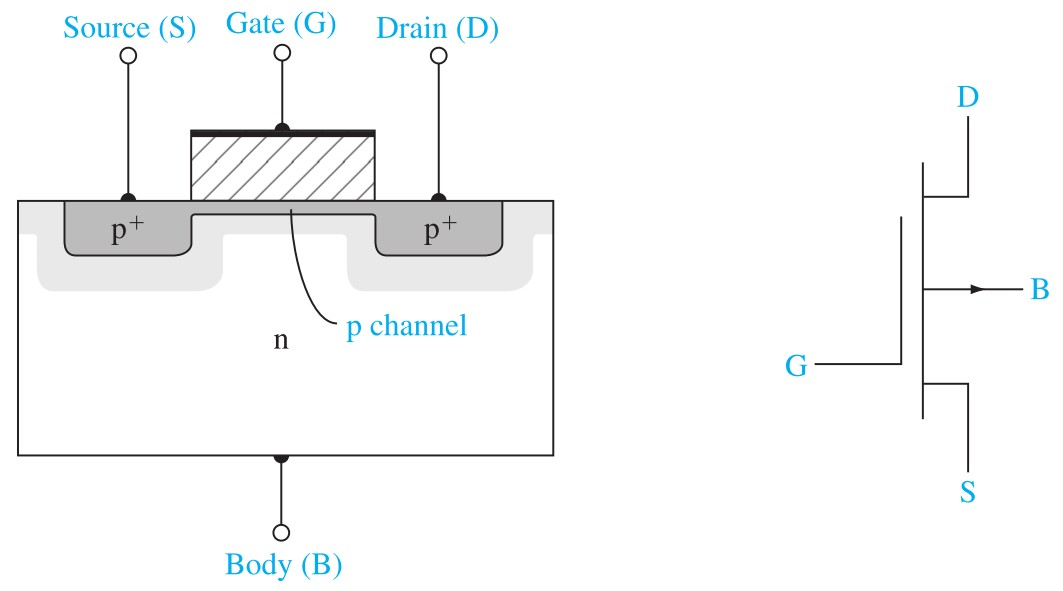
\includegraphics[width=0.9\linewidth]{PMOS-depletion.jpg}
                \caption{p-channel depletion MOSFET}
                \label{subfig:PMOS-depletion.jpg}
            \end{subfigure}
        \end{figure}
    \end{frame}

    \begin{frame} \frametitle{$V_{GS}$ - $V_{T} $}
        \begin{figure}[H]
            \centering
            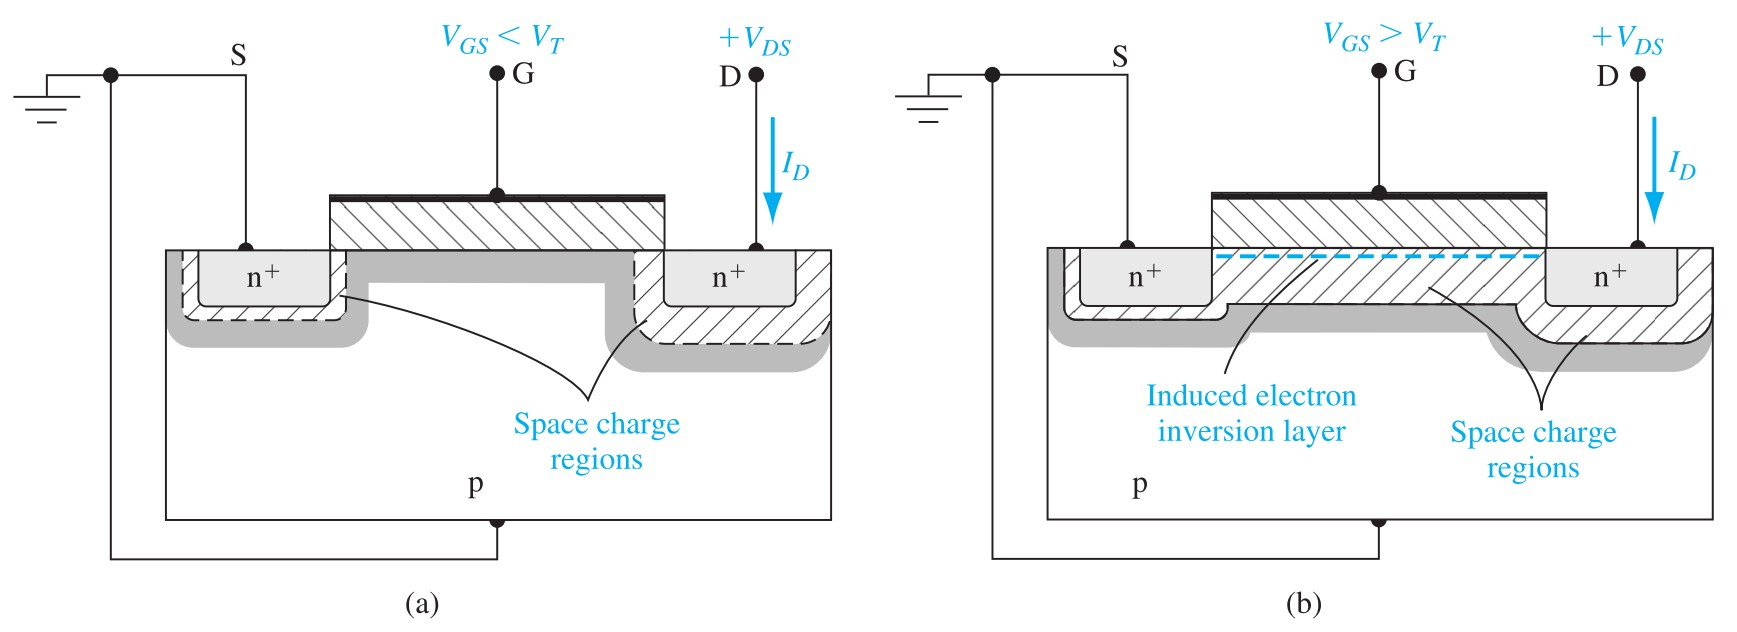
\includegraphics[width=0.9\linewidth]{Current-voltage-relationship.jpg}
            \caption{(a) $V_{GS} < V_T$, (b) $V_{GS} > V_T$}
            \label{fig:Current-voltage-relationship.jpg}
        \end{figure}
        \begin{itemize}
            \item $V_{GS} < V_T$: no inversion layer, no current.
            \item $V_{GS} > V_T$: inversion layer created, current flow from drain to source.
        \end{itemize}
    \end{frame}

    \begin{frame} \frametitle{$V_{DS} $ when $V_{GS} > V_{T} $}
        \begin{itemize}
            \item $V_{DS} $ low ($V_{GS} < V_{GS} - V_T$): act as a controllable resistor.
            \begin{equation*}
                \begin{aligned}
                    \boxed{I_D = \mu_n C_{ox} \frac{W}{L} \left( V_{GS}  - V_T - \frac{V_{DS}}{2}  \right) V_{DS}}
                \end{aligned}
            \end{equation*}
            \item $G_{DS}$ high ($V_{DS} \ge V_{GS} - V_T $): saturation
            \begin{equation*}
                \begin{aligned}
                    \boxed{I_D = \mu_n C_{ox} \frac{W}{2L} \left( V_{GS} - V_T \right)^2 \quad (\text{saturation})}
                \end{aligned}
            \end{equation*}
        \end{itemize}
    \end{frame}

    \begin{frame} \frametitle{$V_{GS}$ - $V_{T} $}
        \begin{figure}[H]
            \centering
            \begin{subfigure}[b]{0.45\linewidth}
                \centering
                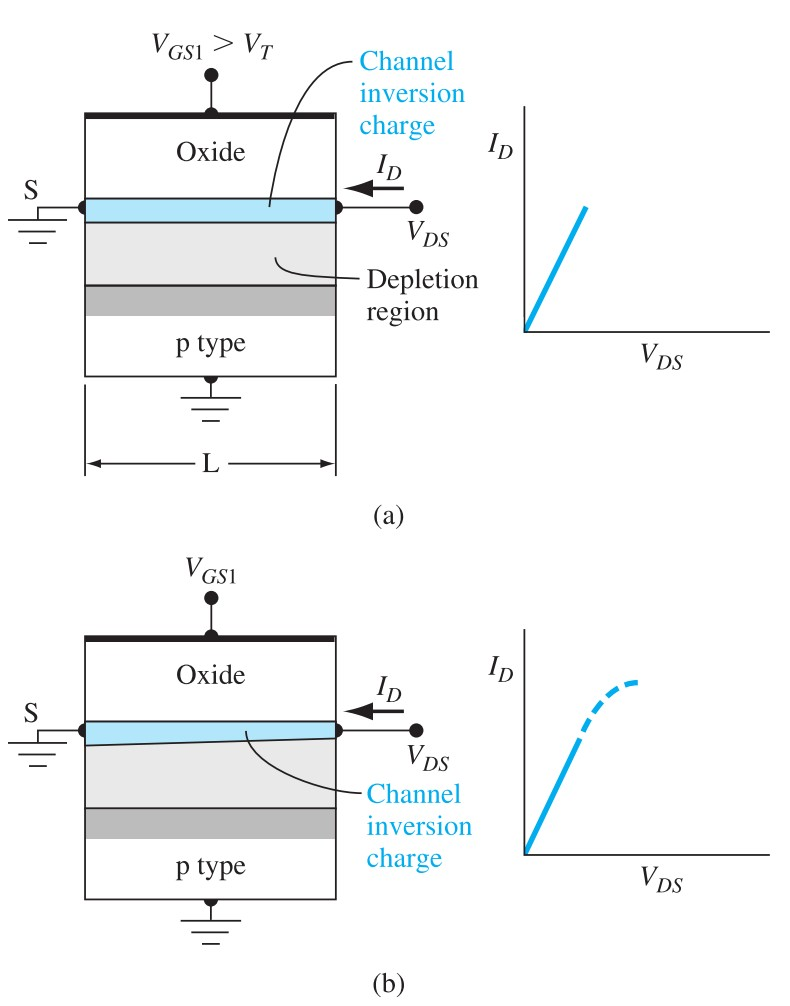
\includegraphics[width=0.9\linewidth]{Vgs-increasing-1.jpg}
                \label{subfig:Vgs-increasing-1.jpg}
            \end{subfigure}
            \begin{subfigure}[b]{0.45\linewidth}
                \centering
                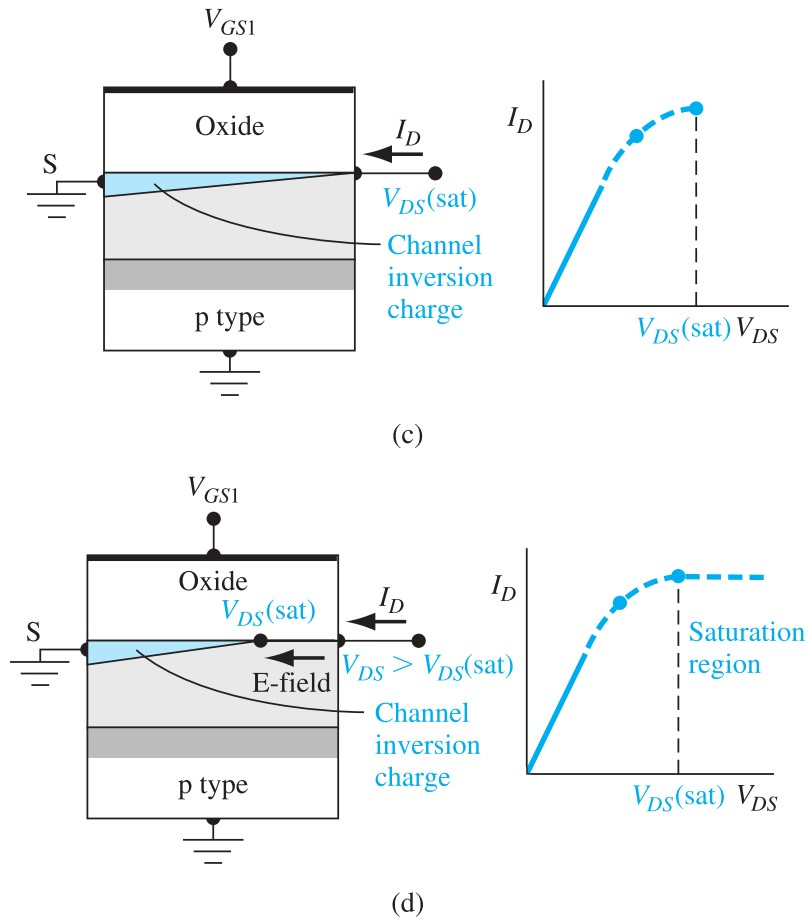
\includegraphics[width=0.9\linewidth]{Vgs-increasing-2.jpg}
                \label{subfig:Vgs-increasing-2.jpg}
            \end{subfigure}
        \end{figure}
        \par After pinch off: the electrons are injected into the space charge region where they are swept by the E-field to the drain contact.
    \end{frame}

    \begin{frame} \frametitle{Transconductance}
        \begin{equation*}
            \begin{aligned}
                g_{m} &= \frac{\partial I_D}{\partial V_{GS} } \\ 
                &= \left\{
                    \begin{aligned}
                        & \mu_n C_{ox} \frac{W}{L} V_{DS} ,\qquad&& 0 < V_{DS} < V_{GS} - V_T \\
                        & \mu_n C_{ox} \frac{W}{L} \left( V_{GS}  - V_T \right) ,\qquad&& V_{DS} > V_{GS} - V_T
                    \end{aligned}
                \right.
            \end{aligned}
        \end{equation*}
    \end{frame}

    \begin{frame} \frametitle{Substrate Bias Effects}
        \begin{figure}[H]
            \centering
            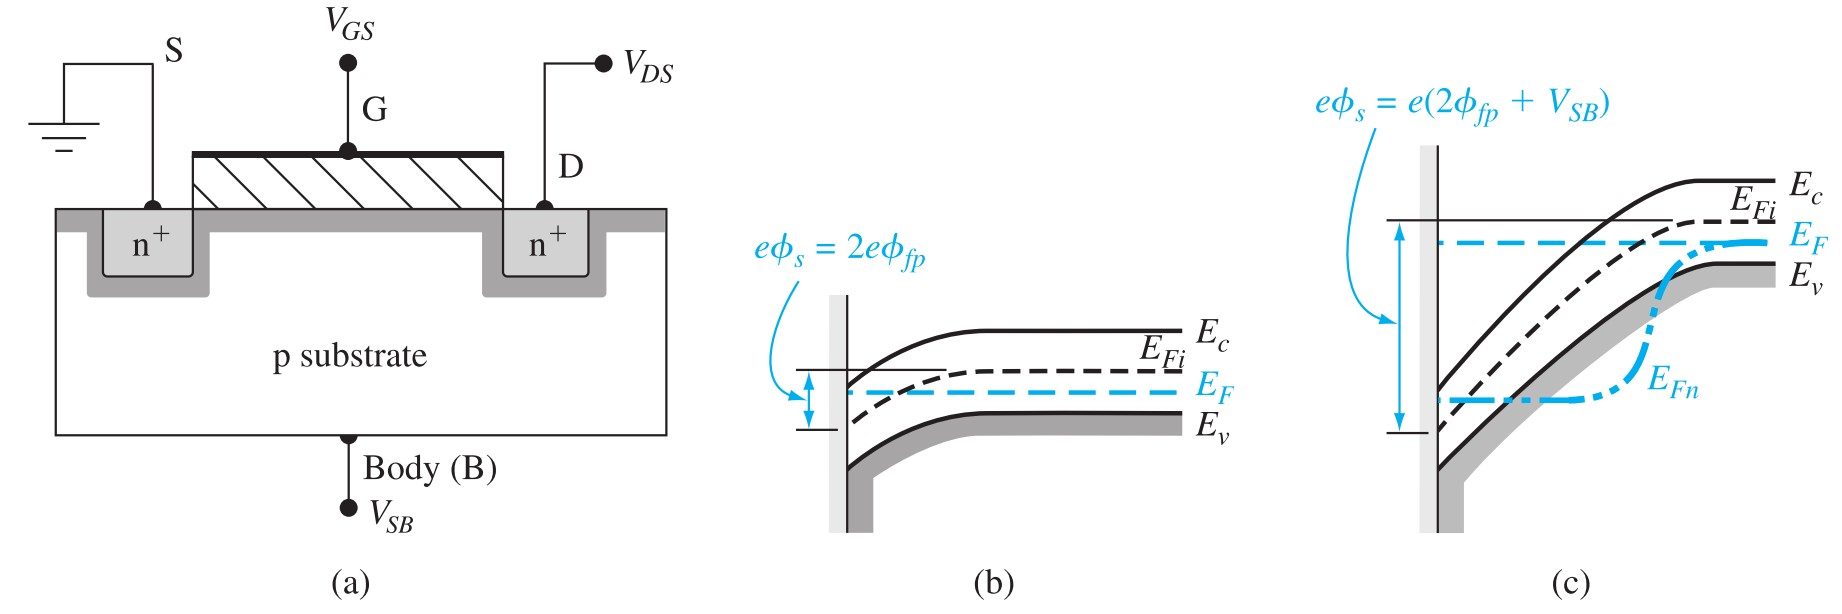
\includegraphics[width=0.9\linewidth]{Substrate-bias-effects.jpg}
            \label{fig:Substrate-bias-effects.jpg}
        \end{figure}
        \begin{equation*}
            \begin{aligned}
                V_{SB} = 0 :\quad & Q^\prime_{SD} (\text{max}) = - \sqrt{2 e \varepsilon_s N_a (2 \phi_{fp} )} \\
                V_{SB} > 0 :\quad & Q^\prime_{SD} = - \sqrt{2 e \varepsilon_s N_a (2 \phi_{fp} + V_{SB} )} \\
            \end{aligned}
        \end{equation*}
        \begin{equation*}
            \boxed{\Delta V_T = - \frac{\Delta Q^\prime_{SD} }{C_{ox} } = \frac{\sqrt{2 e \varepsilon_s N_a}}{C_{ox} }  \left[ \sqrt{2\phi_{fp} + V_{SB}  } - \sqrt{2 \phi_{fp}}\right] }
        \end{equation*}
        where $\Delta V_T = V_T(V_{SB} > 0) - V_{T}(V_{SB} = 0) $ for NMOS.
    \end{frame}
    \begin{frame} \frametitle{Substrate Bias Effects}
        \begin{equation*}
            \boxed{
            \begin{aligned}
                \Delta V_T &= - \frac{\Delta Q^\prime_{SD} }{C_{ox} } = \frac{\sqrt{2 e \varepsilon_s N_a}}{C_{ox} }  \left[ \sqrt{2\phi_{fp} + V_{SB}  } - \sqrt{2 \phi_{fp}}\right] \\
                &= \gamma \left[ \sqrt{2\phi_{fp} + V_{SB}  } - \sqrt{2 \phi_{fp}}\right], \qquad \gamma = \frac{\sqrt{2 e \varepsilon_s N_a}}{C_{ox} }
            \end{aligned}
            }
        \end{equation*}
    \end{frame}

\section{Chapter 11 - Metal–Oxide–Semiconductor Field-Effect Transistor: Additional Concepts}
    \begin{frame} \frametitle{I - Subthreshold Conduction (Leakage Current)}
        \begin{figure}[H]
            \centering
            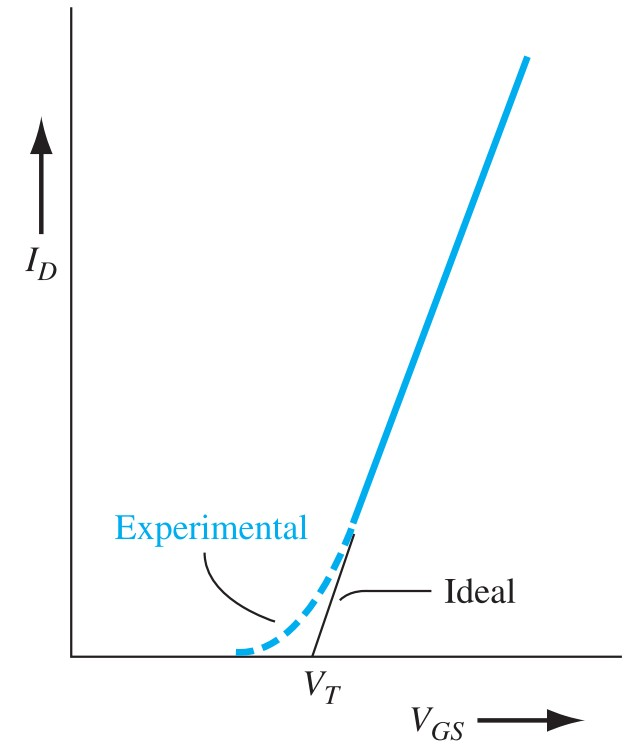
\includegraphics[width=0.4\linewidth]{Subthreshold-condition.jpg}
            \caption{Comparison of ideal and experimental plots of $\sqrt{I_D}$ versus $V_{GS}$.}
            \label{fig:Subthreshold-condition.jpg}
        \end{figure}
        When $V_{GS} < V_T$, $I_D \propto \exp\left( \frac{qV_{GS} }{nkT}  \right)$
    \end{frame}
    \begin{frame} \frametitle{I - Subthreshold Conduction (Leakage Current)}
        Slope Factor: defined to be the inverse slope of the $\log(I_D)$ vs. $V_{GS} $ characteristic in the subthreshold region.
        \begin{figure}[H]
            \centering
            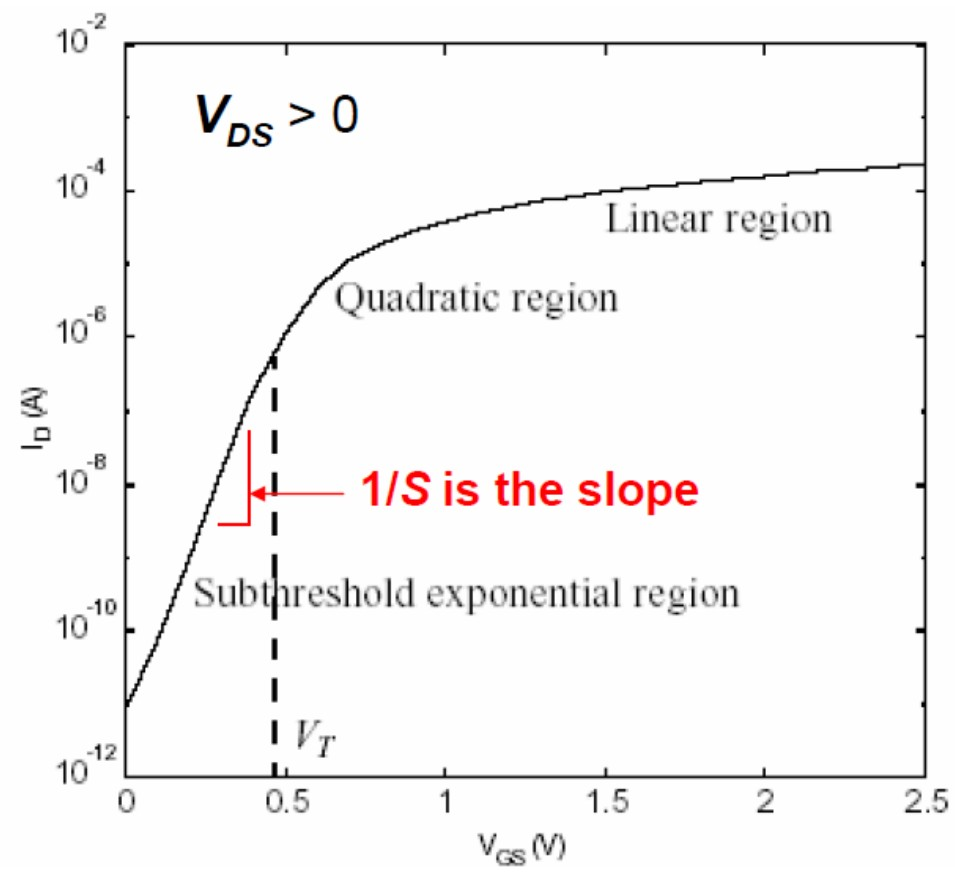
\includegraphics[width=0.6\linewidth]{Slope-factor.jpg}
            \label{fig:Slope-factor.jpg}
        \end{figure}
        \begin{equation*}
            S = n \left( \frac{kT}{q} \ln (10) \right) (\text{Volts per decade})
        \end{equation*}
        \par $S\ge 60 mV/dec$ at room temperature.
    \end{frame}

    \begin{frame} \frametitle{II - Channel Length Modulation}
        \begin{figure}[H]
            \centering
            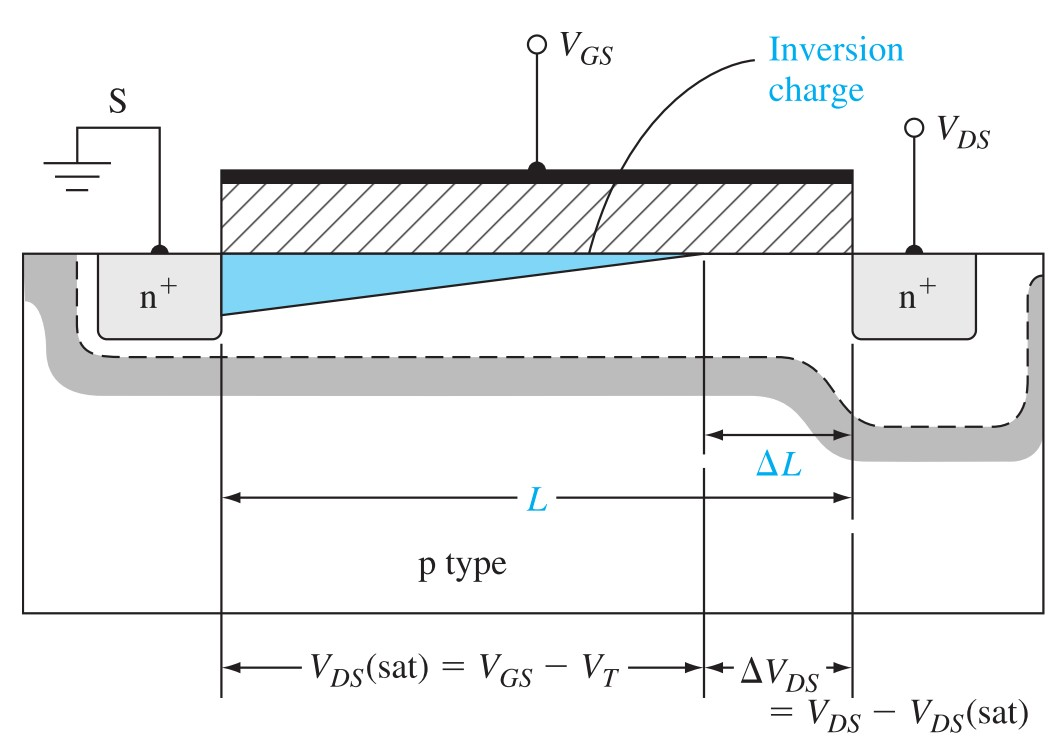
\includegraphics[width=0.6\linewidth]{Channel-length-modulation.jpg}
            \label{fig:Channel-length-modulation.jpg}
        \end{figure}
        \begin{equation*}
            \begin{aligned}
                 I^\prime_D &= \mu_n C_{ox} \frac{W}{2L} \left[\left( V_{GS} - V_T \right)^2  (1 + \lambda V_{DS}) \right] \\
                %  I^\prime_D &= \frac{L}{L - \Delta L} I_D
            \end{aligned}
        \end{equation*}
    \end{frame}

    \begin{frame} \frametitle{III - Velocity Saturation}
        \begin{equation*}
            \begin{aligned}
                I_{DSAT} &= WC_{ox} \left[ V_{GS} - V_{T} - \frac{V_{DSAT} }{2}  \right] v_{sat} \\
            \end{aligned}
        \end{equation*}
        where $V_{DSAT} = \frac{L}{\mu_n} v_{sat}$.
    \end{frame}

    \begin{frame} \frametitle{IV - Short Channel Effect}
        \begin{figure}[H]
            \centering
            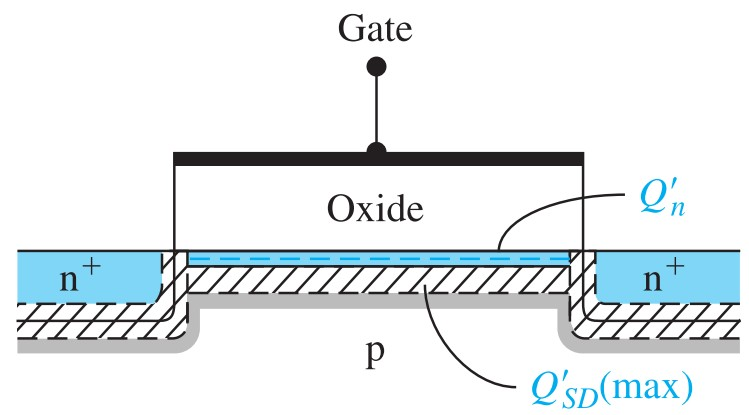
\includegraphics[width=0.4\linewidth]{Short-channel-effects-long-channel.jpg}
            \label{fig:Short-channel-effects-long-channel.jpg}
        \end{figure}
        \begin{figure}[H]
            \centering
            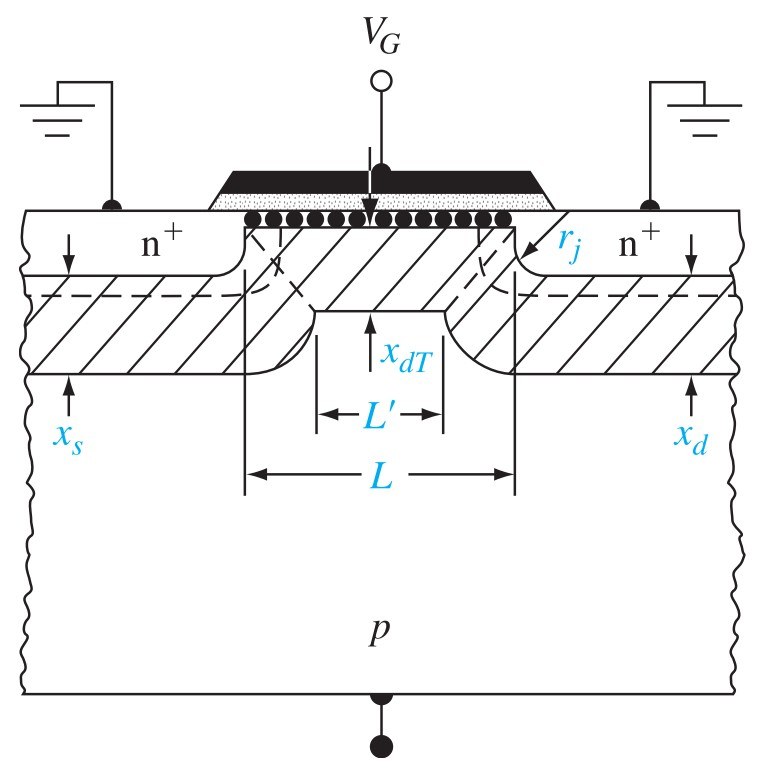
\includegraphics[width=0.5\linewidth]{Short-channel-effects.jpg}
            \label{fig:Short-channel-effects.jpg}
        \end{figure}
    \end{frame}

    % \begin{frame} \frametitle{Exercise}
    %     \par \textcolor{blue}{Objective}: Determine the increase in drain current due to short channel modulation
    %     \par Consider an n-channel MOSFET with a substrate doping concentration of $N_a = 2 \times 10^{16} cm^{-3} $, a threshold voltage of $V_T = 0.4 V$, and a channel length of $L = 1 \mu m$. THe device is biased at $V_{GS} = 1V$ and $V_{DS} = 2.5V$. Determine the ratio of actual drain current compared to the ideal value $I_D^\prime / I_D$. (Example 11.1)
    %     \vspace{1em}
    %     \par \textcolor{blue}{Answer}: \textcolor{white}{1.22} 
    % \end{frame}

    \begin{frame} 
        \begin{center}
            \Large\textcolor{blue}{End}
        \end{center}
    \end{frame}
\end{document} 